\appendix
\chapter{Python skript pro symbolické určení nejistot přísunů radonu}\label{navesti:priloha_nejistoty}
\lstinputlisting[language=Python]{nejistoty.py}

\chapter{Python skript pro vyhodnocení dynamického měření přísunů radonu}\label{navesti:priloha_dynamickeMereni}
\lstinputlisting[language=Python]{dynamickeMereni.py}

\chapter{Přílohy k objektu Skála 75, okr. Havlíčkův Brod}\label{navesti:priloha_skala75}

\section{Fotografie a schéma objektu}

\begin{figure}[H]
    \centering
    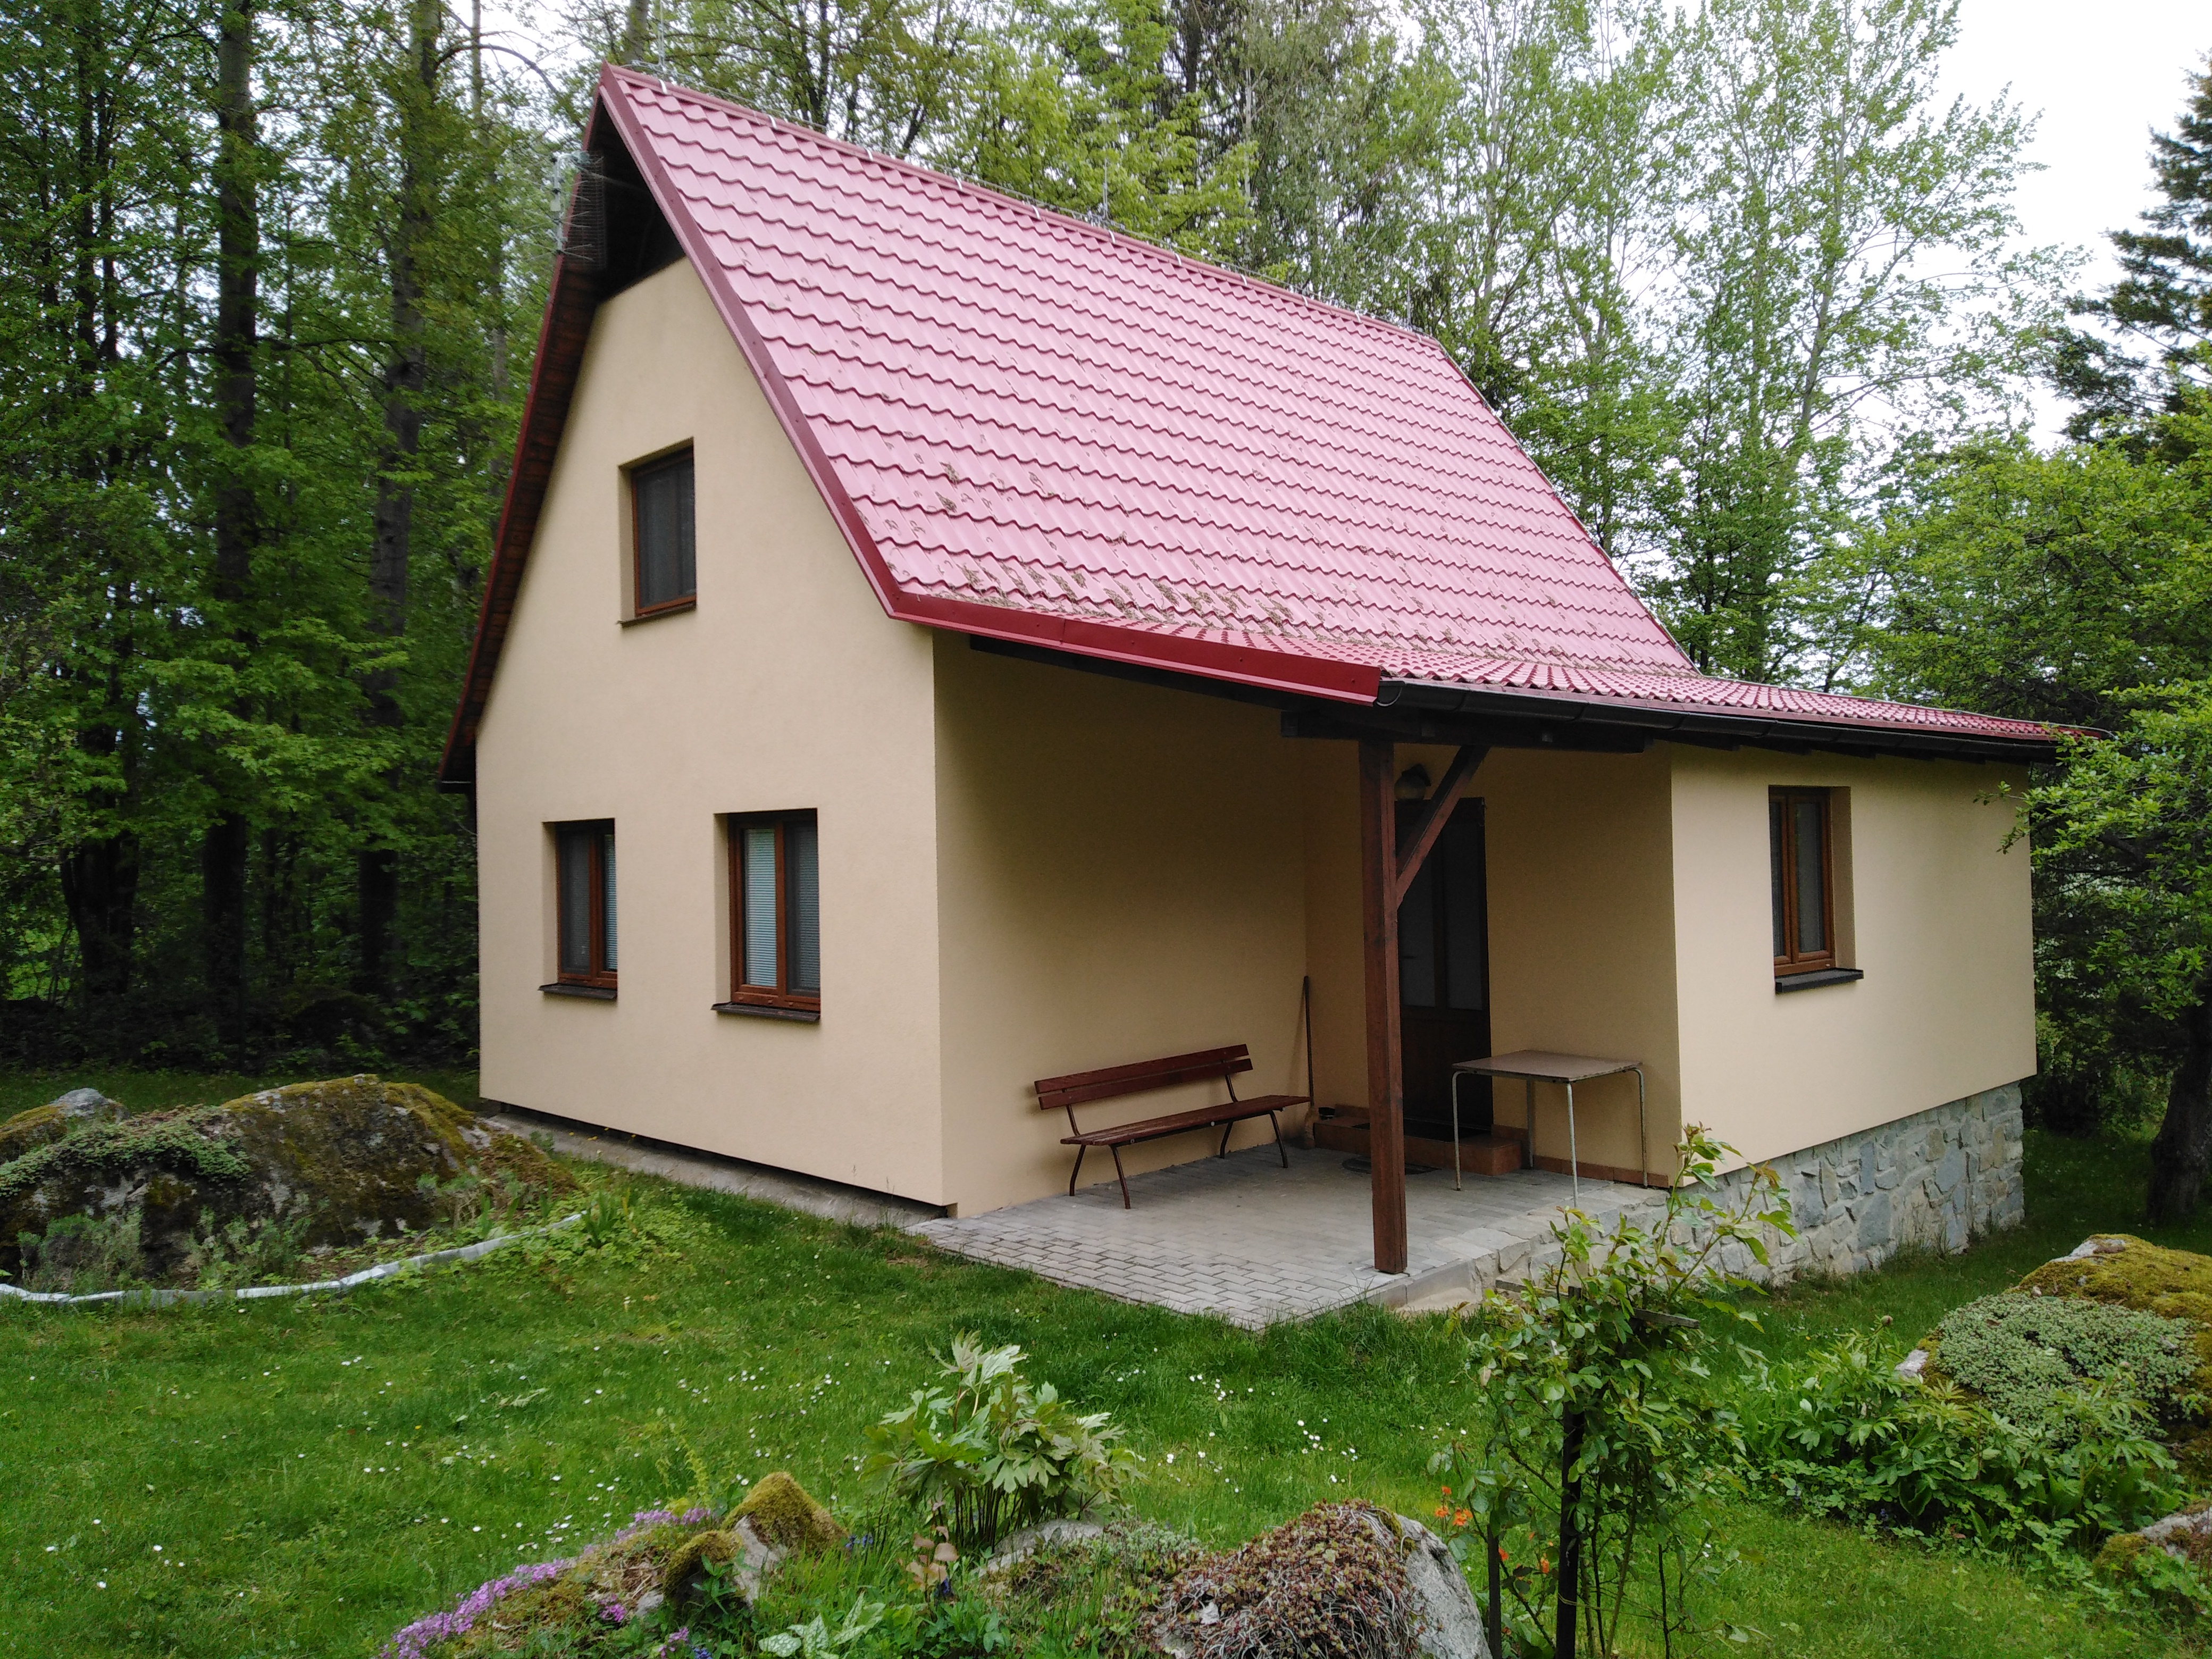
\includegraphics[width=.6\textwidth]{skala75/humpolec_chata.jpg}
    \caption{Fotografie objektu z přední strany.}
    \label{fig:skala75}
\end{figure}

\section{Naměřené vývoje OAR, teplot a relativní vlhkosti vzduchu}

\begin{figure}[H]
    \centering
    %\includegraphics[height=0.8\textwidth, angle=-90, origin=c]{skala75/a1.png}
    \includegraphics[width=1.1\textwidth]{skala75/a1.png}
    \caption{Data z TERA sondy č. 8, která byla umístěna ve sklepě.}
    \label{fig:skala75_a1}
\end{figure}
\begin{figure}[H]
    \centering
    %\includegraphics[height=0.8\textwidth, angle=-90, origin=c]{skala75/a2_1.png}
    \includegraphics[width=1.1\textwidth]{skala75/a2_1.png}
    \caption{Data z TERA sondy č. 10, která byla umístěna v přízemí v kuchyni.}
    \label{fig:skala75_a2_1}
\end{figure}
\begin{figure}[H]
    \centering
    \includegraphics[width=1.1\textwidth]{skala75/a2_2.png}
    \caption{Data z TERA sondy č. 112, která byla umístěna v přízemí v ložnici.}
    \label{fig:skala75_a2_2}
\end{figure}
\begin{figure}[H]
    \centering
    \includegraphics[width=1.1\textwidth]{skala75/a3.png}
    \caption{Data z TERA sondy č. 88, která byla umístěna v prvním patře.}
    \label{fig:skala75_a3}
\end{figure}

\section{Přísuny radonu}

\begin{figure}[H]
    \centering
    \includegraphics[width=\textwidth]{skala75/prisuny1.png}
    \caption{Určený časový vývoj přísunů radonu do jednotlivých podlaží. Nad obrázkem je uvedena kombinace tří použitých indikačních plynů. Oblasti označené zesvětlenou barvou značí nejistotu přísunů radonu při faktoru pokrytí $k=1$.}
    \label{fig:skala75_prisuny1}
\end{figure}
\begin{table}[H]
    \centering
    \caption{Statistiky vypočítaných přísunů radonu $Q$ do jednotlivých podlaží při stejné kombinaci použitých plynů jako v obr. nad touto tabulkou.}
    \label{tab:skala75_prisuny1}
    \begin{tabular}{lrrr}
\toprule
{} &  $Q_0$ $\left[\si{\frac{Bq}{m^3\cdot hod}}\right]$ &  $Q_1$ $\left[\si{\frac{Bq}{m^3\cdot hod}}\right]$ &  $Q_2$ $\left[\si{\frac{Bq}{m^3\cdot hod}}\right]$ \\
\midrule
count &                                                284 &                                                284 &                                                284 \\
mean  &                                                337 &                                                237 &                                                 19 \\
std   &                                                270 &                                                157 &                                                 84 \\
min   &                                                 15 &                                                -85 &                                               -269 \\
25%   &                                                137 &                                                102 &                                                -19 \\
50%   &                                                222 &                                                237 &                                                 -2 \\
75%   &                                                449 &                                                352 &                                                 29 \\
max   &                                               1161 &                                                891 &                                                371 \\
\bottomrule
\end{tabular}

\end{table}

\begin{figure}[H]
    \centering
    \includegraphics[width=\textwidth]{skala75/prisuny2.png}
    \caption{Určený časový vývoj přísunů radonu do jednotlivých podlaží. Nad obrázkem je uvedena kombinace tří použitých indikačních plynů. Oblasti označené zesvětlenou barvou značí nejistotu přísunů radonu při faktoru pokrytí $k=1$.}
    \label{fig:skala75_prisuny2}
\end{figure}
\begin{table}[H]
    \centering
    \caption{Statistiky vypočítaných přísunů radonu $Q$ do jednotlivých podlaží při stejné kombinaci použitých indikačních plynů jako v obr. nad touto tabulkou.}
    \label{tab:skala75_prisuny2}
    \begin{tabular}{lrrr}
\toprule
{} &  $Q_0$ $\left[\si{\frac{Bq}{m^3\cdot hod}}\right]$ &  $Q_1$ $\left[\si{\frac{Bq}{m^3\cdot hod}}\right]$ &  $Q_2$ $\left[\si{\frac{Bq}{m^3\cdot hod}}\right]$ \\
\midrule
count &                                                284 &                                                284 &                                                284 \\
mean  &                                                325 &                                                232 &                                                 64 \\
std   &                                                271 &                                                152 &                                                175 \\
min   &                                                -51 &                                                -85 &                                               -225 \\
25%   &                                                136 &                                                103 &                                                -45 \\
50%   &                                                211 &                                                230 &                                                 -7 \\
75%   &                                                437 &                                                345 &                                                126 \\
max   &                                               1165 &                                                854 &                                                704 \\
\bottomrule
\end{tabular}

\end{table}

\begin{figure}[H]
    \centering
    \includegraphics[width=\textwidth]{skala75/prisuny3.png}
    \caption{Určený časový vývoj přísunů radonu do jednotlivých podlaží. Nad obrázkem je uvedena kombinace tří použitých indikačních plynů. Oblasti označené zesvětlenou barvou značí nejistotu přísunů radonu při faktoru pokrytí $k=1$.}
    \label{fig:skala75_prisuny3}
\end{figure}
\begin{table}[H]
    \centering
    \caption{Statistiky vypočítaných přísunů radonu $Q$ do jednotlivých podlaží při stejné kombinaci použitých indikačních plynů jako v obr. nad touto tabulkou.}
    \label{tab:skala75_prisuny3}
    \begin{tabular}{lrrr}
\toprule
{} &  $Q_0$ $\left[\si{\frac{Bq}{m^3\cdot hod}}\right]$ &  $Q_1$ $\left[\si{\frac{Bq}{m^3\cdot hod}}\right]$ &  $Q_2$ $\left[\si{\frac{Bq}{m^3\cdot hod}}\right]$ \\
\midrule
count &                                                284 &                                                284 &                                                284 \\
mean  &                                               7569 &                                               3802 &                                                393 \\
std   &                                               5260 &                                               2407 &                                                907 \\
min   &                                               1658 &                                                196 &                                               -622 \\
25\%   &                                               3406 &                                               1670 &                                               -161 \\
50\%   &                                               6059 &                                               3494 &                                                -10 \\
75\%   &                                               9630 &                                               5541 &                                                851 \\
max   &                                              22555 &                                               8989 &                                               3053 \\
\bottomrule
\end{tabular}

\end{table}

\begin{figure}[H]
    \centering
    \includegraphics[width=\textwidth]{skala75/prisuny4.png}
    \caption{Určený časový vývoj přísunů radonu do jednotlivých podlaží. Nad obrázkem je uvedena kombinace tří použitých indikačních plynů. Oblasti označené zesvětlenou barvou značí nejistotu přísunů radonu při faktoru pokrytí $k=1$.}
    \label{fig:skala75_prisuny4}
\end{figure}
\begin{table}[H]
    \centering
    \caption{Statistiky vypočítaných přísunů radonu $Q$ do jednotlivých podlaží při stejné kombinaci použitých indikačních plynů jako v obr. nad touto tabulkou.}
    \label{tab:skala75_prisuny4}
    \begin{tabular}{lrrr}
\toprule
{} &  $Q_0$ $\left[\si{\frac{Bq}{hod}}\right]$ &  $Q_1$ $\left[\si{\frac{Bq}{hod}}\right]$ &  $Q_2$ $\left[\si{\frac{Bq}{hod}}\right]$ \\
\midrule
count &                                       284 &                                       284 &                                       284 \\
mean  &                                      7387 &                                      3635 &                                      1086 \\
%std   &                                      5291 &                                      2155 &                                      3010 \\
min   &                                      1578 &                                       232 &                                     -2485 \\
25\%   &                                      3282 &                                      1649 &                                      -700 \\
50\%   &                                      5610 &                                      3423 &                                      -183 \\
75\%   &                                      9590 &                                      5463 &                                      2508 \\
max   &                                     22588 &                                      8028 &                                      9819 \\
\bottomrule
\end{tabular}

\end{table}

\begin{figure}[H]
    \centering
    \includegraphics[width=\textwidth]{skala75/prisuny5.png}
    \caption{Určený časový vývoj přísunů radonu do jednotlivých podlaží. Nad obrázkem je uvedena kombinace tří použitých indikačních plynů. Oblasti označené zesvětlenou barvou značí nejistotu přísunů radonu při faktoru pokrytí $k=1$.}
    \label{fig:skala75_prisuny5}
\end{figure}
\begin{table}[H]
    \centering
    \caption{Statistiky vypočítaných přísunů radonu $Q$ do jednotlivých podlaží při stejné kombinaci použitých indikačních plynů jako v obr. nad touto tabulkou.}
    \label{tab:skala75_prisuny5}
    \begin{tabular}{lrrr}
\toprule
{} &  $Q_0$ $\left[\si{\frac{Bq}{hod}}\right]$ &  $Q_1$ $\left[\si{\frac{Bq}{hod}}\right]$ &  $Q_2$ $\left[\si{\frac{Bq}{hod}}\right]$ \\
\midrule
count &                                       284 &                                       284 &                                       284 \\
mean  &                                      4303 &                                     31307 &                                      1192 \\
std   &                                      3327 &                                     17208 &                                      2931 \\
min   &                                       530 &                                      3155 &                                     -1858 \\
25%   &                                      1769 &                                     14911 &                                      -647 \\
50%   &                                      3058 &                                     31359 &                                       -92 \\
75%   &                                      5563 &                                     44656 &                                      2758 \\
max   &                                     14013 &                                     66567 &                                      9889 \\
\bottomrule
\end{tabular}

\end{table}

\begin{figure}[H]
    \centering
    \includegraphics[width=\textwidth]{skala75/prisuny6.png}
    \caption{Určený časový vývoj přísunů radonu do jednotlivých podlaží. Nad obrázkem je uvedena kombinace tří použitých indikačních plynů. Oblasti označené zesvětlenou barvou značí nejistotu přísunů radonu při faktoru pokrytí $k=1$.}
    \label{fig:skala75_prisuny6}
\end{figure}
\begin{table}[H]
    \centering
    \caption{Statistiky vypočítaných přísunů radonu $Q$ do jednotlivých podlaží při stejné kombinaci použitých indikačních plynů jako v obr. nad touto tabulkou.}
    \label{tab:skala75_prisuny6}
    \begin{tabular}{lrrr}
\toprule
{} &  $Q_0$ $\left[\si{\frac{Bq}{m^3\cdot hod}}\right]$ &  $Q_1$ $\left[\si{\frac{Bq}{m^3\cdot hod}}\right]$ &  $Q_2$ $\left[\si{\frac{Bq}{m^3\cdot hod}}\right]$ \\
\midrule
count &                                                284 &                                                284 &                                                284 \\
mean  &                                                109 &                                                245 &                                                 64 \\
%std   &                                                116 &                                                155 &                                                175 \\
min   &                                               -101 &                                                -80 &                                               -225 \\
25\%   &                                                 32 &                                                108 &                                                -46 \\
50\%   &                                                 74 &                                                247 &                                                 -8 \\
75\%   &                                                162 &                                                361 &                                                125 \\
max   &                                                496 &                                                873 &                                                703 \\
\bottomrule
\end{tabular}

\end{table}

\begin{figure}[H]
    \centering
    \includegraphics[width=\textwidth]{skala75/prisuny7.png}
    \caption{Určený časový vývoj přísunů radonu do jednotlivých podlaží. Nad obrázkem je uvedena kombinace tří použitých indikačních plynů. Oblasti označené zesvětlenou barvou značí nejistotu přísunů radonu při faktoru pokrytí $k=1$.}
    \label{fig:skala75_prisuny7}
\end{figure}
\begin{table}[H]
    \centering
    \caption{Statistiky vypočítaných přísunů radonu $Q$ do jednotlivých podlaží při stejné kombinaci použitých indikačních plynů jako v obr. nad touto tabulkou.}
    \label{tab:skala75_prisuny7}
    \begin{tabular}{lrrr}
\toprule
{} &  $Q_0$ $\left[\si{\frac{Bq}{hod}}\right]$ &  $Q_1$ $\left[\si{\frac{Bq}{hod}}\right]$ &  $Q_2$ $\left[\si{\frac{Bq}{hod}}\right]$ \\
\midrule
count &                                       284 &                                       284 &                                       284 \\
mean  &                                      4539 &                                     26351 &                                      1417 \\
%std   &                                      4571 &                                     17965 &                                      5982 \\
min   &                                     -3147 &                                    -14314 &                                    -18794 \\
25\%   &                                      1499 &                                     11159 &                                     -1311 \\
50\%   &                                      2890 &                                     27642 &                                       -17 \\
75\%   &                                      6434 &                                     39437 &                                      2193 \\
max   &                                     20845 &                                    105191 &                                     26382 \\
\bottomrule
\end{tabular}

\end{table}

\begin{figure}[H]
    \centering
    \includegraphics[width=\textwidth]{skala75/prisuny8.png}
    \caption{Určený časový vývoj přísunů radonu do jednotlivých podlaží. Nad obrázkem je uvedena kombinace tří použitých indikačních plynů. Oblasti označené zesvětlenou barvou značí nejistotu přísunů radonu při faktoru pokrytí $k=1$.}
    \label{fig:skala75_prisuny8}
\end{figure}
\begin{table}[H]
    \centering
    \caption{Statistiky vypočítaných přísunů radonu $Q$ do jednotlivých podlaží při stejné kombinaci použitých indikačních plynů jako v obr. nad touto tabulkou.}
    \label{tab:skala75_prisuny8}
    \begin{tabular}{lrrr}
\toprule
{} &  $Q_0$ $\left[\si{\frac{Bq}{m^3\cdot hod}}\right]$ &  $Q_1$ $\left[\si{\frac{Bq}{m^3\cdot hod}}\right]$ &  $Q_2$ $\left[\si{\frac{Bq}{m^3\cdot hod}}\right]$ \\
\midrule
count &                                                284 &                                                284 &                                                284 \\
mean  &                                               2536 &                                               3929 &                                               1148 \\
std   &                                               1795 &                                               2200 &                                               3007 \\
min   &                                                545 &                                                337 &                                              -2379 \\
25\%   &                                               1145 &                                               1866 &                                               -643 \\
50\%   &                                               1934 &                                               3842 &                                               -135 \\
75\%   &                                               3243 &                                               5850 &                                               2588 \\
max   &                                               7736 &                                               8235 &                                               9876 \\
\bottomrule
\end{tabular}

\end{table}

\chapter{Přílohy k objektu Hálková 980, Humpolec}\label{navesti:priloha_humpolec980}

\section{Schéma objektu}

\section{Naměřené vývoje OAR, teplot a relativní vlhkosti vzduchu}


\chapter{Přílohy k objektu Anglická 574, Dobřichovice}\label{navesti:priloha_anglicka574}

\section{Fotografie a schéma objektu}
\begin{figure}[ht]
    \centering
    \includegraphics[width=.8\textwidth]{anglicka574/dobrichovice.jpg}
    \caption{Fotografie objektu z přední strany.}
    \label{fig:anglicka574_fotografie}
\end{figure}
\section{Naměřené vývoje OAR, teplot a relativní vlhkosti vzduchu}
\begin{figure}[ht]
    \centering
    \includegraphics[width=1\textwidth]{anglicka574/a1.png}
    \caption{Data z TERA sondy č. 8, která byla umístěna ve sklepě.}
    \label{fig:anglicka574_a1}
\end{figure}
\begin{figure}[ht]
    \centering
    \includegraphics[width=1\textwidth]{anglicka574/a2.png}
    \caption{Data z TERA sondy č. 88, která byla umístěna v přízemí.}
    \label{fig:anglicka574_a2}
\end{figure}
\begin{figure}[ht]
    \centering
    \includegraphics[width=1\textwidth]{anglicka574/a3.png}
    \caption{Data z TERA sondy č. 112, která byla umístěna v prvním patře.}
    \label{fig:anglicka574_a3}
\end{figure}

